\documentclass[a4paper, 12pt]{article}
%\documentclass{book}
\usepackage{blindtext}
\usepackage{hyperref}
\usepackage[brazil]{babel}
\usepackage[utf8]{inputenc}
\usepackage{amsmath}
\usepackage{indentfirst}
\usepackage{graphicx}
\usepackage{multicol,lipsum}
\usepackage[a4paper, top=3cm, left=3cm, bottom=3cm, right=3cm]{geometry}
\usepackage{setspace}
\usepackage{multirow}
\usepackage{float}
\usepackage[table]{xcolor}
%\usepackage{pdflscape}
\usepackage[DIV=15]{typearea}
\usepackage[nottoc]{tocbibind}
\usepackage[sort,numbers]{natbib}
%\usepackage{cite}

\documentclass[letterpaper]{article}
% bib pack %%%%%%%%%%%%%%%%%%%%%%%%%%%%%%%%%%%%%%%%%%%%%%%%%%%%%%%%%%%%%%%%%%%%%
\usepackage[utf8]{inputenc}
\usepackage{geometry}
    \geometry{left=3cm,right=2cm,top=2cm,bottom=2cm}
%
\usepackage[spanish]{babel}
%
\usepackage[fixlanguage]{babelbib}
    \bibliographystyle{babunsrt}
%
\usepackage{url}

\begin{document}
%\maketitle

\begin{titlepage}
	\begin{center}
		

\vspace{10pt}
%\begin{figure}[!ht]
%\centering
%
\includegraphics{puc-rio-logo.png}

%\end{figure}
\begin{figure}[!ht]
\centering

\includegraphics{images/puc-rio-logo.png}
\end{figure}
\huge{Laboratório de Controles e Servomecanismos}
        \vspace{70pt}
        
		\textbf{ENG1418}
		\textbf{\large{\\Projeto 3}}
		
		\vspace{30pt}
		\textbf{\small{\\MODELAGEM DE ESPAÇO DE ESTADOS E FUNÇÕES DE TRANSFERÊNCIA}}
		\vspace{65pt}
		
	\end{center}
	
	\begin{flushleft}
		\begin{tabbing}
			Alunos\qquad\qquad\=\>Gabriel Mota Botelho - 1620628\\
			\>Paloma Fernanda Loureiro Sette - 1621595\\
			
			Professor(a)\>Vivian Suzano Medeiros\\
	\end{tabbing}
		  
	\end{flushleft}
	\begin{center}
		%\vspace{\fill}
		Rio de Janeiro, 26 de Abril de 2022
	\end{center}
\end{titlepage}
%%%%%%%%%%%%%%%%%%%%%%%%%%%%%%%%%%%%%%%%%%%%%%%%%%%%%%%%%%%
\newpage
\tableofcontents
\thispagestyle{empty}

\newpage
\pagenumbering{arabic}

\newpage

%\newcommand{\listequationsname}{Lista de Equações}
%\newlistof{myequations}{equ}{\listequationsname}
%\newcommand{\myequations}[1]{%
%\addcontentsline{equ}{myequations}{\protect\numberline{\theequation}#1}\par}

%\listofmyequations
\newpage


\newpage

\listoffigures
\thispagestyle{empty}

\newpage
%%%%%%%%%%%%%%%%%%%%%%%%%%%%%%%%%%%%%%%%%%%%%%%%%%%%%%%%%
%%%%%%%%%%%%%%%%%%%%%%%%%%%%%%%%%%%%%%%%%%%%%%%%%%%
\section{Resumo}

\section{Introdução}



%\section{Sistema Baseado em IoT}
%Esse sistema oferece um mecanismo para detectar cores e classificar itens através do processamento de imagens. Uma vez identificado um mecanismo é usado para classificar qualquer objeto. O sistema usa TCS 3200, que é IoT firmware e conectado a um circuito controlador.

%O TCS 3200 é responsável pela detecção de objetos com base em sua cor e dois servo motores são usados para empurrar ou colocá-los em respectivas caixas.



\section{Sistema Proposto}
A seguir, apresentamos design básico do sistema que estamos propondo:

\begin{figure}[H]
\centering
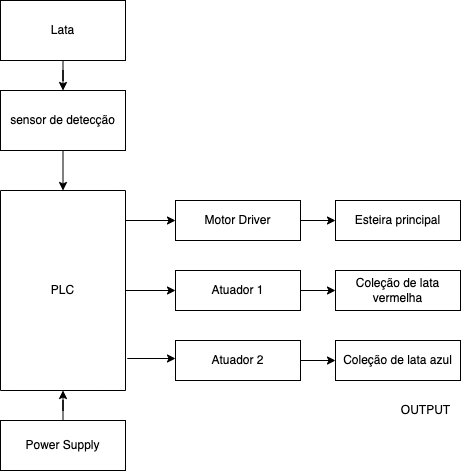
\includegraphics[scale = 0.6]{images/FLUXOGRAMA.png}
\label{filtro1}
\caption{Diagrama de Blocos do Sistema Proposto}
\end{figure}

\begin{figure}[H]
\centering
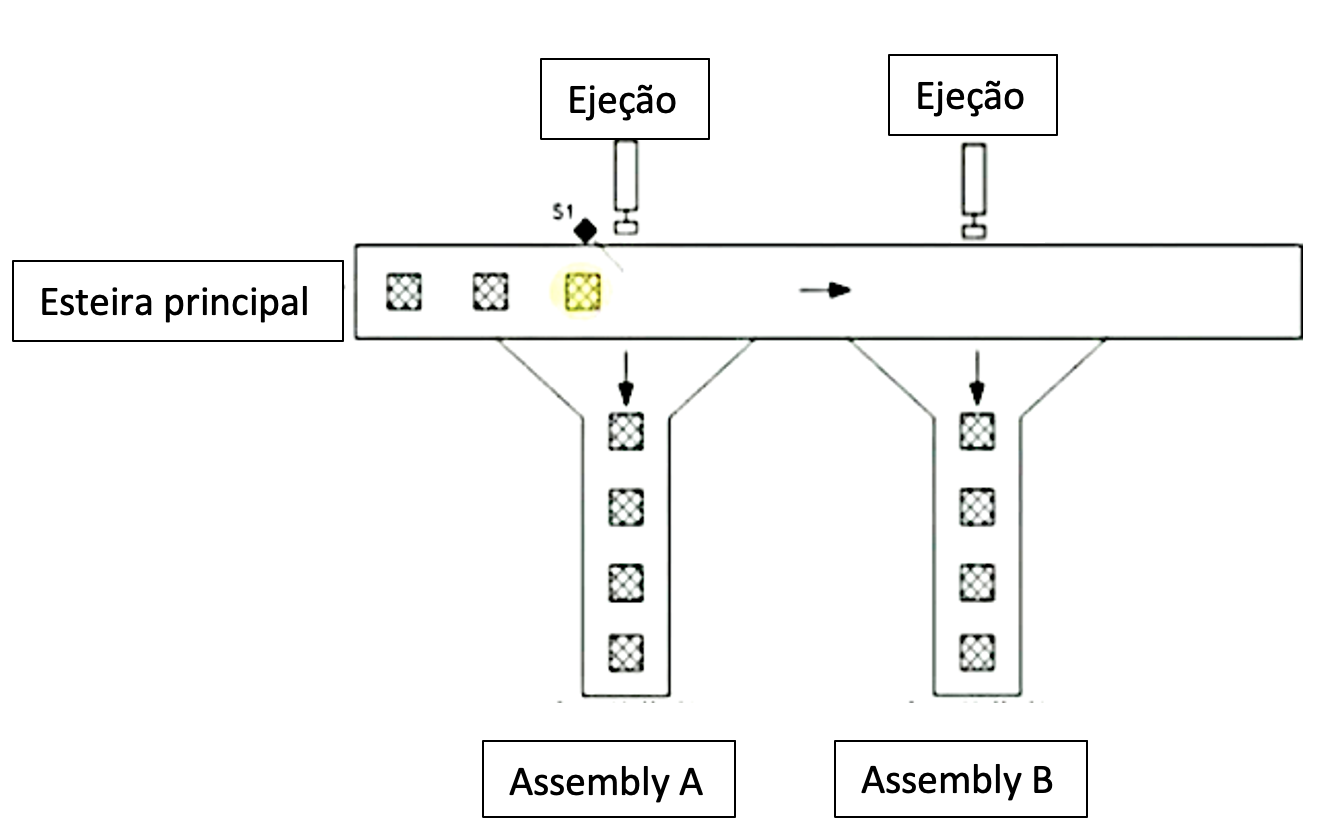
\includegraphics[scale = 0.55]{images/diagramm.png}
\label{filtro1}
\caption{Design inicial proposto}
\end{figure}


Em nosso projeto, temos uma esteira transportadora cujo propósito é encaminhar as latas para a área de destino, de acordo com sua respectiva cor. A correia transportadora as levará para frente da estação de medição de altura. A esteira é executado por \textbf{Motor de indução CA monofásico} controlado por  \textbf{VFD \textit{Variable Frequency Drive}} interfaceado com \textbf{PLC}. O sistema consiste em dois a três racks ou suportes de furos de acordo com o requisito, o 1º mantém um \textbf{sensor LDR}, que iniciará a esteira assim o laser para o LDR for interrompido, e o 2º e 3º suporte seguram um sensor cada, que são organizados para detectar a cor da lata.
Dois atuadores pneumáticos são usados para empurrar as latas nas respectivas caixas de acordo com suas cores.

Quando o feixe de luz para o LDR for cortado pelo objeto, ele sinalizará o PLC para iniciar o transportador principal, por onde as latas são transportadas. Quando as mesmas passam em frente/sob o primeiro sensor, Lx-111-p, o mesmo detectará sua cor. Se a cor for \color{red} \textbf{VERMELHA} \color{black}, enviará  sinal para o PLC e este, por sua vez, alimentará o atuador pneumático responsável por locomover as latas vermelhas, empurrando-as para fora da linha de montagem através do pistão.
Da mesma forma, se o objeto for \color{blue} \textbf{AZUL} \color{black}, o 2º sensor se comportará da mesma forma que o primeiro, no entanto, para a cor azul, sinalizando o PLC para que o segundo atuador tenha a mesma ação que o primeiro, porém, atuando apenas nas latas azuis, a fim de preencher a segunda caixa.

Tivemos a ideia de utilizar o software Factory I/O para uma representação básica e ilustrativa do sistema que estamos propondo. No entanto, vale ressaltar que, para esta representação, tivemos que utilizar os itens gráficos que haviam disponíveis no software, que são placas nas cores verde e azul, para simular as latas. A imagem seguinte demonstra o resultado do design realizado com o software.

\begin{figure}[H]
\centering
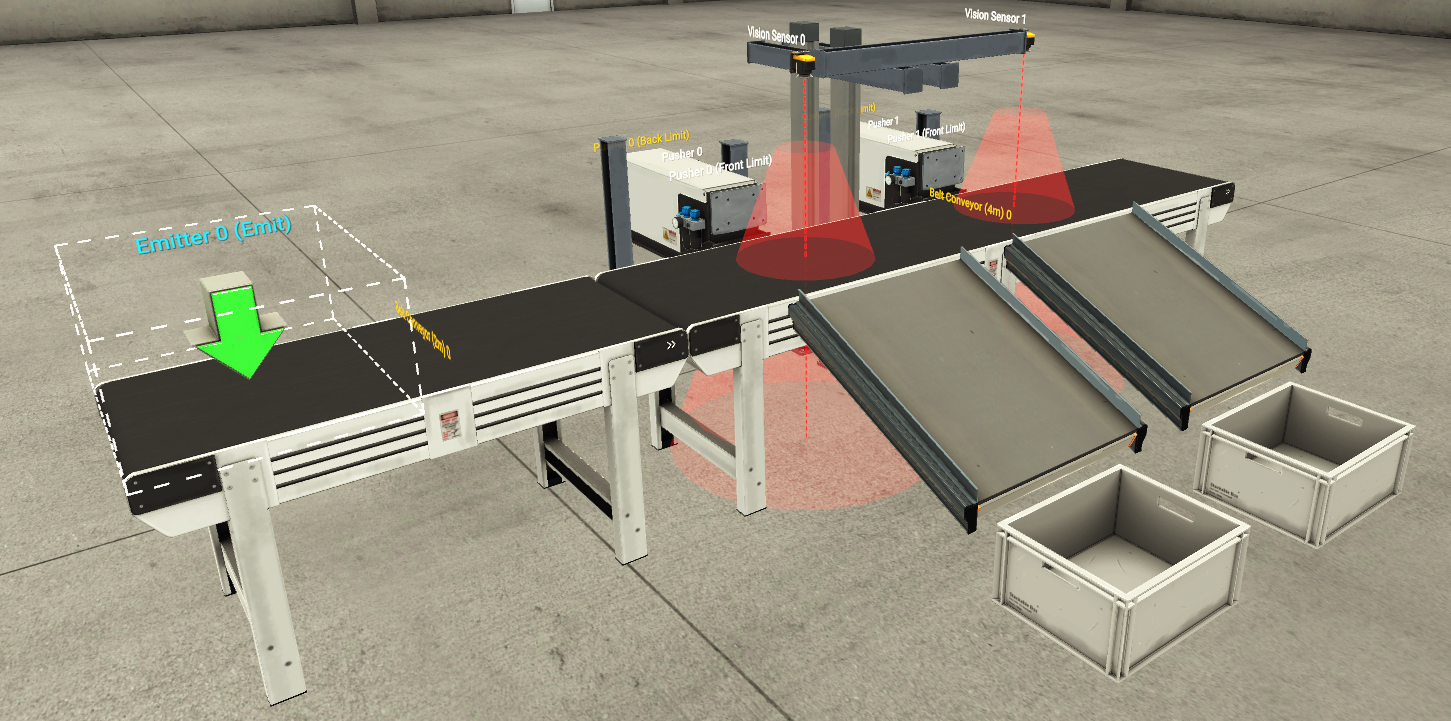
\includegraphics[scale = 0.5]{images/projeto-pronto-esteira.png}
\label{filtro1}
\caption{Design}
\end{figure}

\begin{figure}[H]
\centering
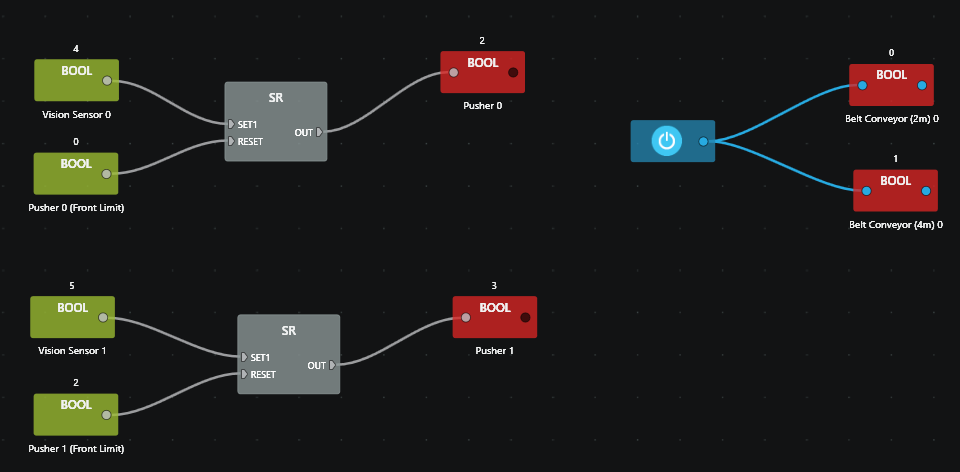
\includegraphics[scale = 0.75]{images/diagrama-factory.png}
\label{filtro1}
\caption{Diagrama de Funcionamento do Projeto pelo Factory I/O}
\end{figure}

Através deste \href{https://www.dropbox.com/s/cchjny23kz1c8tn/separador-latas_lab-servomec-factory-io.mp4?dl=0}{\color{blue}\textbf{link}} é possível visualizar um vídeo demonstrativo do funcionamento do projeto no Factory I/O.

%Através deste \href{http://www.overleaf.com}{link} 

\section{Implementação}
\subsection{PLC}
O PLC é o controlador principal utilizado, sendo usado principalmente para a adaptação dos processos. O PLC consiste da Unidade Central de Processamento (CPU) e sistema de interface (E/S). Este PLC é projetado para realizar operações complexas em escala industrial.

Utilizando sistemas SCADA, o PLC pode ser programado de acordo com o requisito operacional.

\begin{figure}[H]
\centering
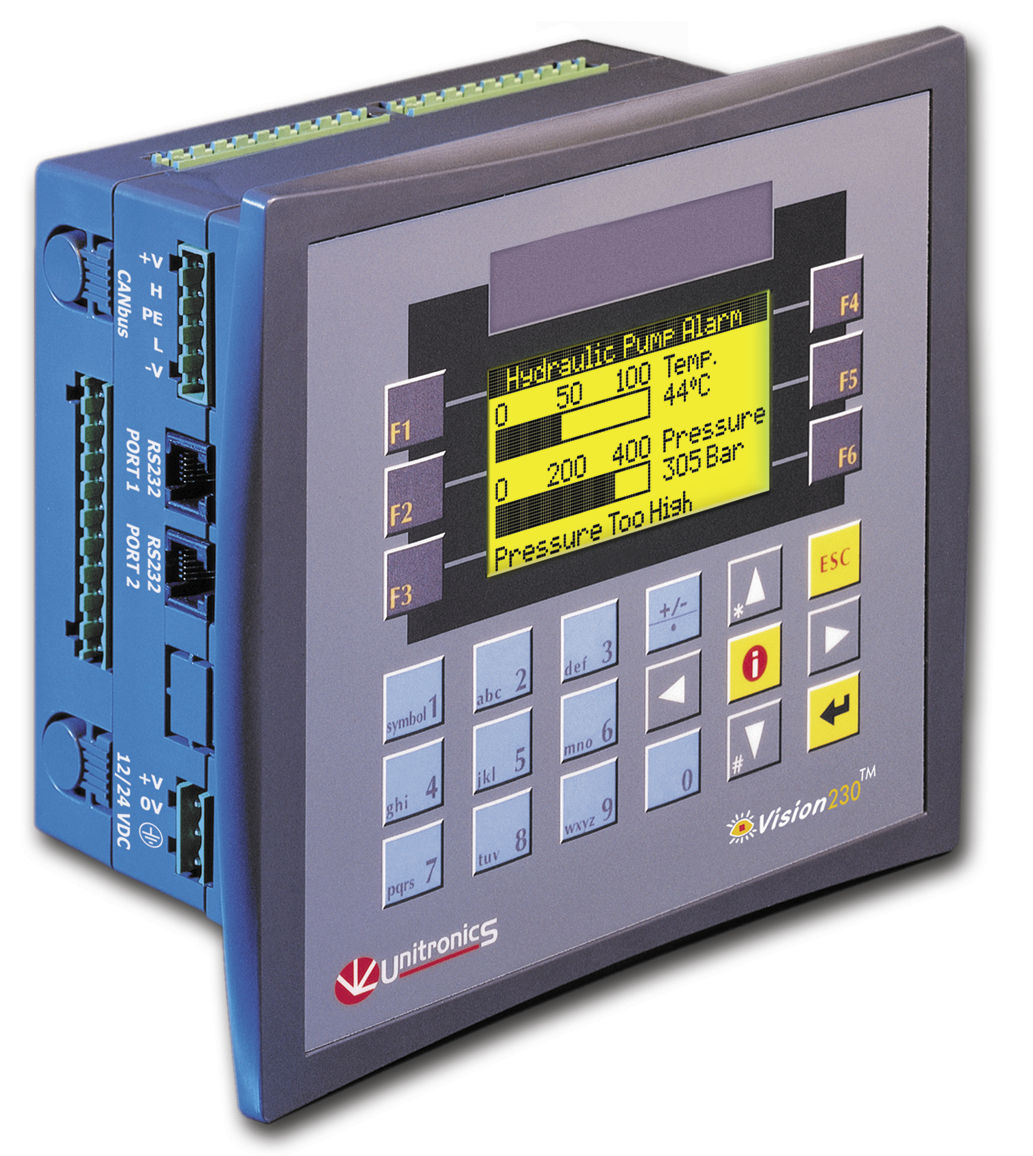
\includegraphics[scale = 0.2]{images/plc.jpeg}
\label{filtro1}
\caption{PLC Display}
\end{figure}

Configurações:
\begin{figure}[H]
\centering
\includegraphics[scale = 0.6]{images/Captura de Tela 2022-04-26 às 17.01.52.png}
\label{filtro1}
\end{figure}

\subsection{Sensor de cor LX-111-P}
O sensor de cor é essencial para garantir o funcionamento adequado de nosso sistema, interagindo com o PLC.
Este sensor é usado para detectar a cor do objeto. É interfaceado com o PLC e a faixa de detecção é de 10 +/- 3mm, 0,394 +/- 0,118 pol. Tensão de alimentação estabelecida na faixa de 12-24 VDC.

\subsection{Esteira Transportadora}
Uma esteira transportadora é essencial para o projeto e é um equipamento comumente usado para transporte contínuo, consistindo em uma alta eficiência e com grande capacidade e abrangência. A montagem é simples e há pouca necessidade de manutenção. Pode ser utilizada para transporte de materiais diversos.

\subsection{Disjuntor (Miniature Circuit Braker - MCB)}
O disjuntor funciona como um interruptor elétrico. Isso significa que é projetado para proteger qualquer tipo de circuito elétrico de danos causados por excesso de corrente de uma sobrecarga ou curto circuito. Há desde pequenos dispositivos para proteger circuitos de baixa corrente ou grandes dispositivos para proteger os circuitos domésticos. A principal função de um disjuntor é agir como um dispositivo de proteção para o sistema.

\subsection{Motor de Indução Trifásico (assíncrono)} 
Uma das vantagens do motor de indução AC é que ele é ideal para operação unidirecional e bi-direcional, como esteiras e sistemas de transporte de carga.

\subsubsection{Modo Vetorial de Controle}
possibilita atingir um elevado grau de precisão e rapidez no controle do torque e da velocidade do motor. O controle decompõe a corrente do motor em dois vetores: um que produz o fluxo magnetizante e outro que produz torque, regulando separadamente o torque e o fluxo. O controle vetorial pode ser realizado em malha aberta (“sensorless”) ou em malha fechada (com realimentação). Embora o controle por malha aberta seja mais simples que o controle com sensor, há limitações de torque principalmente em baixíssimas rotações. Em velocidades maiores é praticamente tão bom quanto o controle vetorial com realimentação. 

Portanto, requer a instalação de um sensor de velocidade (por exemplo, um \textbf{encoder incremental}) no motor. Este tipo de controle permite a maior precisão possível no controle da velocidade e do torque, inclusive em rotação zero.

\subsection{Encoder Incremental}
codificador ou transdutor de posição angular, fornece medidas e controles de forma precisa em velocidade de rotação, velocidade linear, posicionamento angular ou linear do motor.
Gerando informações de posição, ângulo e números de rotação, que são definidas com base no número de pulsos por rotação, retransmitidos pelo encoder ao comando para cada rotação. A seguir, o comando determina a posição atual por meio da contagem destes pulsos.

\subsection{Relay}
Usado para conectar ou desconectar dois circuitos, funcionando como um interruptor, no entanto, sem operação manual. Podemos encontrar de diversos tipos, como eletromecânicos, que são frequentemente utilizados. Para nosso projeto, nos interessa as seguintes especificações:

i. Alta capacidade, relé de baixo perfil.

ii. Baixa potência da bobina de 400mW.

\subsection{Atuadores Elétricos Lineares}
Fabricado com fusos trapezoidais  e chaves “limits switches” internas que permitem o atuador linear elétrico parar automaticamente ao alcançar o fim de curso de modo a proteger contra eventuais aquecimentos.

Controle de Posição:
Se precisarmos de controle de posição, a solução já embarcada no atuador é o uso do potenciômetro interno  0-10K, que permite o controle de posição externo através de um sinal analógico 0-10V.

Controle de velocidade:
Possui com um Motor de Ímã permanente DC e variar a velocidade é muito simples com o uso da Placa de chaveamento PWM.

\section{Fluxograma de Funcionamento}
Abaixo, demonstramos o fluxograma relativo às ações do sistema proposto:

\begin{figure}[H]
\centering
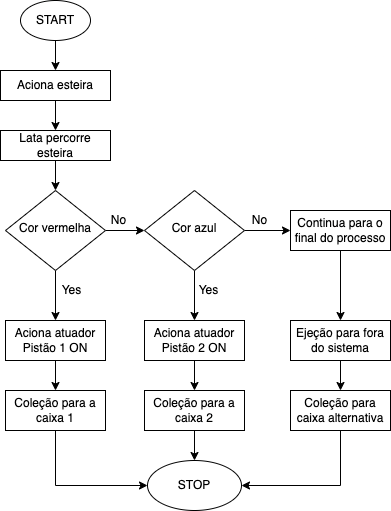
\includegraphics[scale = 0.7]{images/fluxograma2.png}
\label{filtro1}
\caption{Fluxograma do sistema}
\end{figure}

\section{Conclusão}
A partir dos levantamentos que fizemos,  observamos que as metodologias convencionais para classificar um objeto por cor são, de fato, ineficientes. Considerando que o sistema que idealizamos reduz o fator tempo, bem como
trouxe mais precisão numa linha de montagem. Não é apenas economia de tempo, mas também reduz a necessidade de ações humanas nas operações de triagem que, em última análise, reduzem custo da operação.

A gestão da integridade de fornecimento de um produto, desde a matéria-prima até o produto acabado, através da fabricação de qualidade é de suma importância para a geração de um produto com alta qualidade e precisão. Então, este projeto de classificação automática de cores é pertinente devido ao seu princípio de funcionamento e ampla implementação. Ao aplicar a ideia deste projeto, podemos facilmente classificar o produto necessário de acordo com
sua cor. Embora haja algumas limitações, este conceito pode ser implementado em ampla gama de aplicações.

\newpage

% REFERENCIAS %%%%%%%%%%%%%%%%%%%%%%%%%%%%%%%%%%%%%%%%%%%%%%%%%%%%%%%%%%%%%%
    \nocite{*}
    \bibliography{src/bibliography}
    
\end{document}
\section{Referências Bibliográficas}

\end{document}